\section{Initial frontier-model evaluations}
\label{sec:evals}

We evaluate twelve model configurations against HLG, drawn from the model list in
\texttt{model\_list.txt}. Six base models, each at \texttt{none} and \texttt{high}
reasoning effort:

\begin{itemize}[leftmargin=1.5em]
    \item \texttt{claude-sonnet-4-6}
    \item \texttt{claude-opus-4-6}
    \item \texttt{gpt-5.4}
    \item \texttt{gpt-5.4-nano}
    \item \texttt{oai-gpt-5-2-2025-12-11}
    \item \texttt{oai-gpt-4.1-2025-04-14}
\end{itemize}

\subsection{Evaluation regimes}

For each model we report results in three regimes:
\begin{enumerate}[leftmargin=1.5em]
    \item \textbf{Turn (parallel).} 34 levels run in parallel, each level with an
      isolated session and accumulating conversation history within attempts.
    \item \textbf{Turn (sequence).} 34 levels run sequentially with prior level
      attempts injected into the next level's first user message via
      \texttt{<level\_history>}.
    \item \textbf{One-shot.} The model emits a full move sequence per attempt; no
      intermediate observations are provided.
\end{enumerate}

\subsection{Results}

Per-model HLG-RHAE values, level-completion counts, and total token usage are reported in
Table~\ref{tab:leaderboard} (in Section~\ref{sec:measuring}). Figure~\ref{fig:perf}
visualizes the cost--RHAE Pareto frontier across configurations.

\begin{figure}[t]
    \centering
    % Auto-generated by scripts/build_paper_assets.py
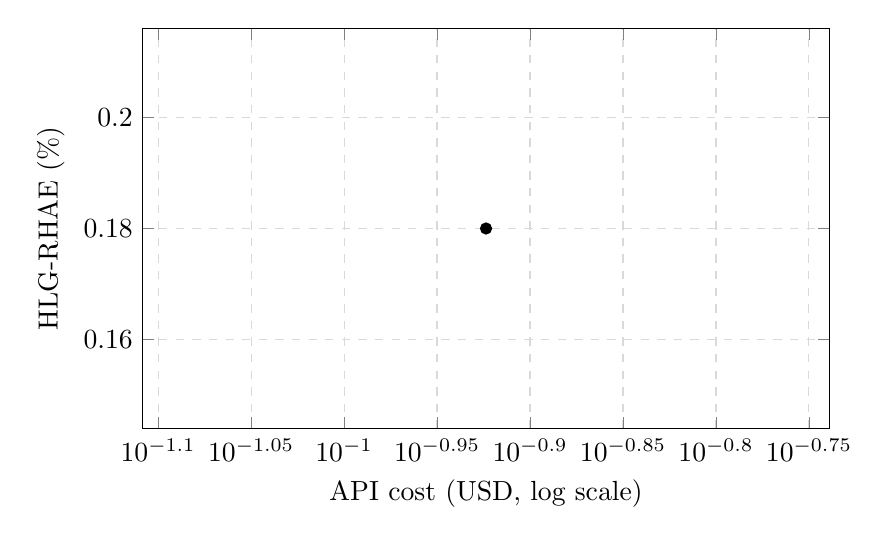
\begin{tikzpicture}
\begin{axis}[
    width=0.85\linewidth, height=0.55\linewidth,
    xmode=log,
    xlabel={API cost (USD, log scale)},
    ylabel={HLG-RHAE (\%)},
    grid=both,
    grid style={dashed, gray!30},
    only marks,
    nodes near coords,
    nodes near coords align={above},
    point meta=explicit symbolic,
]
\addplot[mark=*, mark size=2pt] coordinates {
        (0.1192, 0.1800)
};
\end{axis}
\end{tikzpicture}

    \caption{HLG-RHAE versus dollar cost across the evaluated configurations (turn
    mode, official leaderboard). Each point is a (model, reasoning-effort) pair.
    Dollar cost is computed from per-token rates published by each provider as of
    March 2026 (see \texttt{scripts/build\_paper\_assets.py} for the rate table). The
    pgfplots source is auto-generated from \texttt{data/leaderboard.json}; rerun
    \texttt{python scripts/build\_paper\_assets.py} to refresh.}
    \label{fig:perf}
\end{figure}

\subsection{Qualitative findings}

\paragraph{Loss vs.\ dead state.} Across configurations, frontier models routinely fail
to distinguish a legal-but-unwinnable state from an illegal move. They activate a
\texttt{close} switch that closes the only required bridge, then continue planning as
if the future were unconstrained. Models receive an explicit \texttt{[DEAD]} tag in
their next-attempt context; this often is not enough to identify the earlier branching
point that caused the dead end.

\paragraph{Weak-tile orientation.} Models often correctly avoid \emph{landing} upright
on a weak tile, but fail to plan a flat traversal of a weak-tile corridor when an
upright landing would otherwise be the most direct path.

\paragraph{Split mode.} Two-target teleport levels separate two halves of the block.
Frontier models in our evaluation rarely succeed on these levels, often outputting the
\texttt{s} action outside of split mode (which is a no-op) or failing to plan for the
merge geometry.

\paragraph{One-shot vs turn.} One-shot mode is materially cheaper but its WIN rate
is uniformly lower than turn mode at matched compute. The gap is largest on levels
with bridge-group toggling, where online correction in turn mode lets the model
recover from a misjudged switch order.
